\documentclass[11pt,a4paper]{article}
\usepackage[T1]{fontenc}
\usepackage[utf8]{inputenc}
\usepackage{newtxtext,newtxmath,microtype}
\usepackage[margin=22mm,headheight=14pt]{geometry}
\usepackage{booktabs,tabularx,array,caption,float,amsmath,tikz}
\usepackage{listings}
\usepackage{xcolor,fancyhdr,lastpage}
\usepackage[hidelinks]{hyperref}
\definecolor{accent}{HTML}{254C58}
\hypersetup{pdftitle={Section 1 -- Cable selection and model setup},pdfauthor={Tiebert Lefebure}}
\pagestyle{fancy}\fancyhf{}
\fancyhead[L]{\small Finite Elements for Electromagnetic Fields}
\fancyhead[R]{\small 33 kV NKT cable}
\fancyfoot[L]{\small Section 1: Cable selection and model setup}
\fancyfoot[R]{\small \thepage\,/\,\pageref{LastPage}}
\renewcommand{\headrulewidth}{0.3pt}
\setlength{\parindent}{0pt}\setlength{\parskip}{4pt}
\setlength{\intextsep}{4pt}
\setlength{\emergencystretch}{1em}
\setlength{\tabcolsep}{6pt}\renewcommand{\arraystretch}{1.12}
\captionsetup{font=small,labelfont=bf,skip=5pt}
\newcolumntype{Y}{>{\raggedright\arraybackslash}X}
\newcommand{\source}[2]{\href{#1}{#2}}
\newcommand{\codefile}[1]{\href{run:#1}{\nolinkurl{#1}}}
\lstset{basicstyle=\footnotesize\ttfamily,numberstyle=\tiny\color{black!60},
  numbers=left,numbersep=8pt,xleftmargin=16pt,columns=fullflexible,
  keepspaces=true,showstringspaces=false,breaklines=true,upquote=true,
  aboveskip=6pt,belowskip=6pt}
\lstdefinestyle{command}{numbers=none,basicstyle=\small\ttfamily,
 backgroundcolor=\color{accent!5},aboveskip=4pt,belowskip=5pt,
 xleftmargin=5pt,xrightmargin=5pt,breaklines=true}
\newcommand{\guidetitle}{\par\smallskip{\small\bfseries\color{accent}Code guide}\par}
\newcommand{\codeguide}[3]{%
 \begingroup\small\setlength{\tabcolsep}{0pt}\renewcommand{\arraystretch}{1.1}%
 \begin{tabularx}{\linewidth}{@{}p{20mm}Y@{}}
 \textbf{Computes} & #1\\[2pt]
 \textbf{Read} & #2\\[2pt]
 \textbf{Inspect} & #3
 \end{tabularx}\par\endgroup\smallskip}
% Generated by Source-code/section_1/calculate_geometry.py.
\newcommand{\ContactThickness}{1.651}
\newcommand{\CopperThickness}{0.399}
\newcommand{\CopperInnerRadius}{19.751}
\newcommand{\BundleDiameter}{98.039}

% Original question wording: NMES Assignment 2026, Sections 1 and 2.
% Line-wrap hyphenation is removed; mathematical notation is typeset in LaTeX.
\usepackage{tcolorbox}
\newcommand{\assignmentquestion}[1]{%
  \begin{tcolorbox}[colback=accent!4,colframe=accent!65,
    boxrule=0pt,leftrule=2pt,arc=0pt,boxsep=0pt,
    left=7pt,right=7pt,top=5pt,bottom=5pt,
    before skip=0pt,after skip=8pt,fontupper=\small]
  \textbf{Assignment question.} #1
  \end{tcolorbox}%
}
\newcommand{\questionfiles}[1]{%
  \par\smallskip{\footnotesize\color{accent}
  \textbf{Files / results (relative to Source-code).} #1\par}\medskip
}
\newcommand{\QuestionOneOne}{%
Describe your cable: construction, dimensions, materials, rated voltage, rated
current (ampacity) and the laying conditions for which that rating is given
(burial depth, soil thermal resistivity, ambient temperature, arrangement).
Give a table of electromagnetic and thermal properties with a source for each value.}
\newcommand{\QuestionOneTwo}{%
Choose the environment consistently with the datasheet rating conditions,
and justify its properties.}
\newcommand{\QuestionOneThree}{%
State the sheath bonding you assume: single-point bonded (no net sheath current)
or solidly bonded (circulating sheath currents allowed), and how the armour
and pipe are connected. This choice strongly affects the losses in Section 3.}
\newcommand{\QuestionOneFour}{%
State the excitation you impose: phase-to-ground voltage and phase current,
as peak phasors, with the phase sequence (see the conventions in Appendix A).}
\newcommand{\QuestionTwoOne}{%
Define your computational domain, the equations solved and the boundary
conditions. Where do you truncate the domain, and why? Discuss the role of
the grounded screens: which regions actually influence the field in the insulation?}
\newcommand{\QuestionTwoTwo}{%
Can you simplify the geometry of your cable without degrading the precision
(e.g. disregard details in the geometrical description)? Quantify the effect
of each simplification.}
\newcommand{\QuestionTwoThree}{%
How do the results vary with the mesh refinement? Plot the maximum field in
the insulation and the capacitance versus the number of degrees of freedom,
and identify where local refinement is needed.}
\newcommand{\QuestionTwoFour}{%
Define the admissible field strength at the conductor screen and at the core
screen from the datasheet (or, if absent, from a cited reference).
Is the healthy cable within these limits?}
\newcommand{\QuestionTwoFive}{%
Add a defect to the insulation of your cable. State its nature (e.g. gas void,
water tree, protrusion of the semiconducting screen), its properties, size and
position, and discuss what a defect in a 2D cross-section represents in 3D.
Compare the field with and without defect along a radial cut.
Does the cable withstand the defect?}
\newcommand{\QuestionTwoSix}{%
Compute the resistive and displacement current densities in the cable.
Is current conservation satisfied? Which current dominates in each material, and why?}
\newcommand{\QuestionTwoSeven}{%
Compute the per-unit-length capacitance (\(\mu\mathrm{F/km}\)) and compare with
the analytical value (13) and with the datasheet. State the assumptions of the
analytical formula (in particular, how the semiconducting layers are treated).
Does the capacitance vary with frequency? Why (not)?}
\newcommand{\QuestionTwoEight}{%
Propose an improvement of the cable design with respect to the electric stress,
and support it quantitatively.}

\begin{document}

\section*{Q1.1 Cable construction and dimensions}
\assignmentquestion{\QuestionOneOne}
Run the question commands from \path{Source-code/section_1} using Python 3.
Paths in the code guides are relative to that folder. No Gmsh or GetDP solve is required.
\guidetitle
\begin{lstlisting}[style=command]
python3 calculate_geometry.py
\end{lstlisting}
\codeguide
 {Layer radii, copper-ring thickness and effective aluminium conductivity.}
 {\path{cable_inputs.json} supplies dimensions; \path{calculate_geometry.py} checks and converts them.
  \path{../shared/materials.json} supplies material constants.}
 {\path{derived_geometry.json}: \texttt{phase\_radii\_mm} follows Table~\ref{tab:phase};
  \texttt{aluminium\_effective\_sigma\_20\_S\_m} is in S/m.}
We model three NKT 33 kV XLPE-AL single-core cables, each with a nominal
\(240~\mathrm{mm^2}\) aluminium conductor and \(50~\mathrm{mm^2}\) copper
screen [1]. For direct burial in touching trefoil with both ends bonded, NKT
gives \(415~\mathrm A\) RMS. Installation conditions are given in
Table~\ref{tab:rating}.

Each cable has a solid circular aluminium conductor, semiconducting screens
on both sides of the XLPE, a copper wire screen with counter-wound tape, and
its own PE sheath. There is no armour, common jacket or pipe.

\begin{table}[H]\centering\small
\caption{Radial model of one cable. Radii are measured from the conductor axis.}
\label{tab:phase}
\begin{tabularx}{\linewidth}{@{}Y r r l@{}}
\toprule
Region & Thickness [mm] & Outer radius [mm] & Source\\
\midrule
Aluminium conductor & --- & 8.500 & NKT [1]\\
Inner semiconductor & 0.800 & 9.300 & Assumed from [2]\\
XLPE insulation & 8.000 & 17.300 & NKT [1]\\
Outer semiconductor & 0.800 & 18.100 & Assumed from [2]\\
Equivalent contact region & \ContactThickness & \CopperInnerRadius & Calculated\\
Equivalent copper screen & \CopperThickness & 20.150 & Area from [1]\\
Equivalent PE outer cover & 2.600 & 22.750 & Diameter from [1]\\
\bottomrule
\end{tabularx}
\end{table}

\textbf{Missing dimensions.} NKT does not specify the semiconducting-screen
thicknesses. We use \(0.8~\mathrm{mm}\) for each, from the 33 kV specification
OES 2 [2]. The inner value matches the listed diameter over XLPE:
\(17.0+2(0.8)+2(8.0)=34.6~\mathrm{mm}\). The screens smooth the electrical
interfaces; the inner-screen thickness sets the XLPE radii and affects the
field and capacitance.

We replace the individual copper wires and tape by a continuous circular
ring. We keep the specified copper area and the diameter over the screen,
\(40.3~\mathrm{mm}\). With \(r_o=20.15~\mathrm{mm}\), the inner radius is
\[
 A_{\mathrm{Cu}}=\pi(r_o^2-r_i^2)=50~\mathrm{mm^2},\qquad
 r_i=\sqrt{r_o^2-50/\pi}=\CopperInnerRadius~\mathrm{mm}.
\]
Lines 20--21 of \texttt{calculate\_geometry.py} implement this approximation:
\lstinputlisting[language=Python,firstline=20,lastline=21,firstnumber=20]{../../Source-code/section_1/calculate_geometry.py}
The ring is therefore \(\CopperThickness~\mathrm{mm}\) thick. The remaining
\(\ContactThickness~\mathrm{mm}\) between the outer semiconductor and copper
is represented by a contact region with semiconducting properties. This keeps
the insulation screen electrically connected to the copper. The ring preserves
copper area but omits individual wires and helical paths, so detailed screen
currents and losses remain approximate. Assigning one thermal conductivity
to the contact region also approximates heat flow through the wire and tape
construction.

\newpage
\section*{Q1.1 Material properties (continued)}
The screen and cable diameters imply a cover of
\((45.5-40.3)/2=2.6~\mathrm{mm}\), compared with the listed \(2.3~\mathrm{mm}\)
PE sheath. We use the \(2.6~\mathrm{mm}\) effective cover to retain the outside
diameter, assigning the unspecified \(0.3~\mathrm{mm}\) PE properties. This
also affects the cover's thermal resistance.

The electrical constants are stored in
\codefile{Source-code/shared/materials.json}; the full set of material
properties is given below. The sources are the datasheet, literature and
assignment. Each region is homogeneous and isotropic, with scalar properties
that are initially constant.

\begin{table}[H]\centering\small
\caption{Material properties used in the initial model. Metal conductivities are at \(20^\circ\mathrm C\).}
\label{tab:materials}
\begin{tabularx}{\linewidth}{@{}Y c c c c l@{}}
\toprule
Material & \(\varepsilon_r\) & \(\mu_r\) &
\(\sigma~[\mathrm{S/m}]\) & \(\kappa~[\mathrm{W/(m\,K)}]\) & Source\\
\midrule
Aluminium & 1 & 1 & \(3.52454\times10^7\) & 237 & [1,5], see below\\
Copper & 1 & 1 & \(5.95\times10^7\) & 402 & [5]\\
Semiconducting PE & 2.25 & 1 & \(2\times10^{-3}\) & 0.286 & [2,5]\\
XLPE & 2.5 & 1 & \(10^{-18}\) & 0.286 & [6,7]\\
PE outer cover & 2.25 & 1 & \(10^{-18}\) & 0.46 & [8]\\
Soil & 10 & 1 & \(10^{-2}\) & 0.83333 & [1,A]\\
\bottomrule
\end{tabularx}
\end{table}

We take \(\mu_r=1\) for all regions. In metals, conduction current dominates
at 50 Hz, so using \(\varepsilon_r=1\) has little influence. Both screens and
the contact region use the same semiconducting properties.

\subsection*{Aluminium conductivity}
The \(17.0~\mathrm{mm}\) conductor diameter gives an area of
\(\pi(8.5)^2=226.98~\mathrm{mm^2}\), rather than the nominal
\(240~\mathrm{mm^2}\). We keep the listed diameter and choose an effective
conductivity from the maximum DC resistance of \(0.125~\Omega/\mathrm{km}\)
at \(20^\circ\mathrm C\):
\[
 R=\frac{\ell}{\sigma A},\qquad
 \sigma_{\mathrm{Al},20}
 =\frac{1000}{0.125\,\pi(0.0085)^2}
 =3.52454\times10^7~\mathrm{S/m}.
\]
This matches the datasheet's maximum resistance, rather than a measured
resistance of a particular cable. The thermal conductivity is taken
separately from [5].

\subsection*{Semiconducting screens and insulation}
The chosen screen conductivity, \(0.002~\mathrm{S/m}\), corresponds to a
resistivity of \(500~\Omega\,\mathrm m\), the insulation-screen limit at
\(90^\circ\mathrm C\) in [2]. We use it as a constant estimate since the
NKT compound data are unavailable. At 50 Hz,
\(\sigma/(\omega\varepsilon)\approx3.2\times10^5\), so the screens conduct
well relative to the XLPE and have very little voltage drop across them.
This motivates checking an equipotential-screen approximation in Section 2.

XLPE has a very small conductivity; its permittivity mainly determines the
electric field and charging current. The PE cover insulates the copper from
the soil. We use a real, constant permittivity and omit dielectric loss
tangent, so the model does not capture the full dielectric heating of the
real cable.

\subsection*{Temperature dependence}
We first use constant properties. For the coupled thermal calculation, the
metal conductivities are updated with temperature using Appendix A [A]:
\[
 \sigma(T)=\frac{\sigma_{20}}{1+\alpha(T-20^\circ\mathrm C)},\qquad
 \alpha_{\mathrm{Cu}}=0.00386~\mathrm{K^{-1}},\quad
 \alpha_{\mathrm{Al}}=0.00390~\mathrm{K^{-1}}.
\]
As temperature rises, conductivity decreases and Joule losses increase for
the same current. The nonmetallic properties are kept constant. In particular,
the model does not account for changes in soil moisture or drying.

\newpage
\section*{Q1.2 Installation and environment}
\assignmentquestion{\QuestionOneTwo}
\guidetitle
\begin{lstlisting}[style=command]
python3 calculate_geometry.py
\end{lstlisting}
\codeguide
 {Touching-trefoil phase positions and axis depths, taking burial depth to the centroid.}
 {Installation and soil inputs are in \path{cable_inputs.json}.
  In \path{calculate_geometry.py}, \texttt{centres} sets the
  local coordinates and \texttt{depths} converts them to depths below ground.}
 {\path{derived_geometry.json}:
  \texttt{phase\_centres\_relative\_to\_centroid\_mm} is in mm;
  \texttt{phase\_axis\_depths\_m} is in m. Check A above B and C.}
We use the direct-burial conditions of NKT's \(415~\mathrm A\) rating [1].
The three PE sheaths touch, with phase A above phases B and C. Thus the
centre-to-centre distance is the cable diameter, \(D=45.5~\mathrm{mm}\).

\begin{figure}[H]\centering
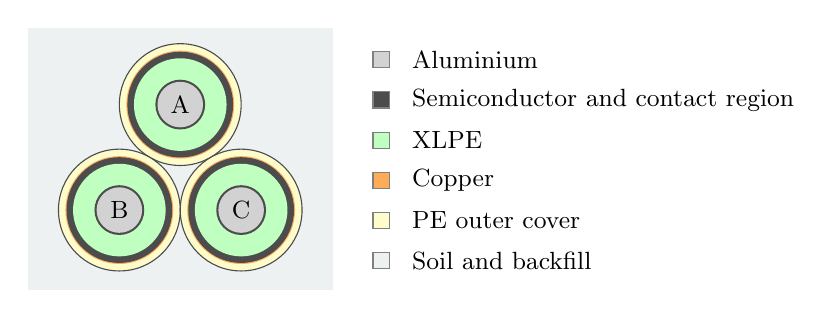
\begin{tikzpicture}[x=0.034cm,y=0.034cm,font=\small]
\fill[accent!8] (-57,-43) rectangle (57,55);
\foreach \x/\y/\name in {0/26.26944/A,-22.75/-13.13472/B,22.75/-13.13472/C}{
 \filldraw[fill=yellow!20,draw=black!70] (\x,\y) circle (22.75);
 \fill[orange!65] (\x,\y) circle (20.15);
 \fill[black!70] (\x,\y) circle (19.75113);
 \fill[green!25] (\x,\y) circle (17.3);
 \fill[black!70] (\x,\y) circle (9.3);
 \fill[gray!35] (\x,\y) circle (8.5);
 \node at (\x,\y) {\name};
}
\foreach \col/\y/\name in {gray!35/43/Aluminium,black!70/28/Semiconductor and contact region,green!25/13/XLPE,orange!65/-2/Copper,yellow!20/-17/PE outer cover,accent!8/-32/Soil and backfill}{
 \filldraw[fill=\col,draw=black!50] (72,\y-3) rectangle (78,\y+3);
 \node[anchor=west] at (83,\y) {\name};
}
\end{tikzpicture}
\caption{Cross-section of the touching trefoil. The ground surface is above the drawing.}
\end{figure}

The local origin is the trefoil centroid and \(y\) is positive upwards.
The centres are at \((0,D/\sqrt3)\) and
\((\pm D/2,-D/(2\sqrt3))\). The enclosing-circle diameter is
\(D(1+2/\sqrt3)=\BundleDiameter~\mathrm{mm}\); this is only a measure of
the bundle size, not an additional boundary or layer.

\begin{table}[H]\centering\small
\caption{Installation conditions and phase positions.}
\label{tab:rating}
\begin{tabularx}{\linewidth}{@{}l Y@{}}
\toprule
Quantity & Value used\\
\midrule
Voltage and reference current [1] & 33 kV line-to-line RMS; 415 A RMS per phase\\
Screen bonding [1] & Both ends bonded\\
Burial depth [1] & 1.0 m; taken to the trefoil centroid\\
Soil temperature and resistivity [1] & \(15^\circ\mathrm C\); \(1.2~\mathrm{K\,m/W}\)\\
Maximum conductor temperature [1] & \(90^\circ\mathrm C\)\\
Phase A: position; depth & \((0,26.269)~\mathrm{mm}\); \(0.974~\mathrm m\)\\
Phase B: position; depth & \((-22.750,-13.135)~\mathrm{mm}\); \(1.013~\mathrm m\)\\
Phase C: position; depth & \((22.750,-13.135)~\mathrm{mm}\); \(1.013~\mathrm m\)\\
\bottomrule
\end{tabularx}
\end{table}

The datasheet does not define the reference for burial depth, so we take
\(1.0~\mathrm m\) to the centroid. We use
\(\kappa_{\mathrm{soil}}=1/1.2=0.83333~\mathrm{W/(m\,K)}\).
The electrical soil properties in Table~\ref{tab:materials} are the example
values from Appendix C [A], used in the absence of site data.

We treat soil and backfill as one uniform region, including the small space
between the three cables. Prepared bedding and restraints are typical of
trefoil installations [3,4], but are not modelled separately. We assume good
contact between soil and jackets, with no air gaps or contact thermal
resistance. Poor contact or dry soil would increase the conductor temperature.

The 2D model represents a long, straight cable with the same cross-section
along its length. End effects, joints and local restraints are omitted;
longitudinal conductor currents are still included. The thermal calculation
must later include heat transfer to the ground surface and check the effect
of domain size. At \(415~\mathrm A\), the hottest conductor temperature is
then compared with the \(90^\circ\mathrm C\) limit. The datasheet rating
still needs thermal validation.

\newpage
\section*{Q1.3 Screen bonding}
\assignmentquestion{\QuestionOneThree}
\guidetitle
\begin{lstlisting}[style=command]
python3 -m json.tool cable_inputs.json
\end{lstlisting}
\codeguide
 {No FE calculation: the command displays the saved inputs so the bonding choice can be checked.}
 {\texttt{screen\_bonding} in \path{cable_inputs.json} records the choice.
  \texttt{Constraint} in \path{../section_2/cable.pro} grounds the screens;
  \texttt{GradientConstraint} in \path{../section_3/model.pro} sets their axial voltage gradient.}
 {The value \texttt{both\_ends\_ideal\_common\_earth}.
  This is an input assumption; Section 3 solves the resulting screen currents.}
We assume that each copper screen is connected to a common earth at both
ends, as in the selected rating row. The bonding leads and earth connections
have zero impedance in the model. The PE jackets insulate the screens from
the soil and from each other along the cable. There is no armour or pipe to
connect.

For the electric model, the copper screen potential is set to zero. The inner
semiconductor follows the conductor potential, while the outer semiconductor
is connected to the copper through the equivalent contact region.

For the magnetic model, both-end bonding allows a circulating current to
flow in each screen. We impose zero longitudinal voltage per unit length,
and solve for the resulting net screen current:
\[
 \frac{\widehat{\mathcal U}_m}{\ell}=0,\qquad
 \widehat I_m=\int_{\Omega_m}\widehat J_z\,\mathrm dS.
\]
Here \(\Omega_m\) is the copper region of screen \(m\). Its current can be
nonuniform, so local eddy currents are also allowed. These currents produce
additional Joule losses and must be included in the heat source. For
single-point bonding the net screen current would instead be zero, although
local eddy currents could remain. This is why the bonding assumption matters
for the losses.

\newpage
\section*{Q1.4 Excitation}
\assignmentquestion{\QuestionOneFour}
\guidetitle
\begin{lstlisting}[style=command]
python3 calculate_geometry.py
\end{lstlisting}
\codeguide
 {Phase-to-ground peak voltage from line-to-line RMS voltage, and peak current from RMS current.}
 {\path{cable_inputs.json} supplies voltage, current and frequency.
  Lines 53--54 of \path{calculate_geometry.py} perform the amplitude conversions.}
 {\path{derived_geometry.json}:
  \texttt{peak\_phase\_voltage\_V} and \texttt{peak\_phase\_current\_A}.
  These are amplitudes; the ABC angles are applied in the FE models below.}
We use a balanced three-phase system at \(f=50~\mathrm{Hz}\), with positive
sequence ABC. Phase A is the top cable, B the lower left cable and C the lower
right cable. Following Appendix A [A], phasors represent peak values:
\[
 x(t)=\Re\{\widehat x\,e^{\mathrm j\omega t}\},\qquad \omega=2\pi f.
\]
The rated voltage is line-to-line RMS. Its phase-to-ground RMS value is
\(33/\sqrt3=19.053~\mathrm{kV}\), giving the peak amplitudes
\[
 V_{\mathrm{pk}}=\sqrt{\frac23}\,33=26.944~\mathrm{kV},\qquad
 I_{\mathrm{pk}}=\sqrt2\,415=586.899~\mathrm A.
\]
The corresponding lines 53--54 of \texttt{calculate\_geometry.py} are:
\lstinputlisting[language=Python,firstline=53,lastline=54,firstnumber=53]{../../Source-code/section_1/calculate_geometry.py}

\begin{table}[H]\centering
\caption{Imposed peak phasors. Voltages are phase-to-ground.}
\begin{tabular}{@{}c c c@{}}
\toprule
Phase & Voltage [kV] & Current [A]\\
\midrule
A & \(26.944\angle0^\circ\) & \(586.899\angle0^\circ\)\\
B & \(26.944\angle(-120^\circ)\) & \(586.899\angle(-120^\circ)\)\\
C & \(26.944\angle(+120^\circ)\) & \(586.899\angle(+120^\circ)\)\\
\bottomrule
\end{tabular}
\end{table}

We assume unity power factor, so each phase current is in phase with its
voltage. The voltages excite the electric model and the net conductor currents
excite the magnetic model. The screen currents follow from the magnetic
solution and the bonding conditions; they are not prescribed as part of the
three-phase excitation.

{\small
\textbf{In the FE models.} \codefile{Source-code/section_2/cable.pro} applies
the voltage phasors and \codefile{Source-code/section_3/model.pro} applies
the conductor current phasors. Each section's \texttt{prepare.py} reads the
same inputs and writes \texttt{parameters.inc} in SI units. The command above
only calculates amplitudes; solver runs belong to Sections 2 and 3.\par}

\newpage
\section*{References}
\begingroup\small\setlength{\parskip}{10pt}
[1] NKT, \textit{33 kV single core cable XLPE-AL Halogen free}, printed
pp.~19--20, \(240~\mathrm{mm^2}\) column. Cable construction, dimensions,
DC resistance and current ratings.
\source{https://nkt.widen.net/content/d8gut55fhb/pdf/33kV_1-core_XLPE-AL-RMP-FB-ST_CU_screen_DSENAPP_MV_DS_EN.pdf?u=gj0n1y}{Manufacturer datasheet}.

[2] Authority for Public Services Regulation, Oman, \textit{OES 2: Cables and
Accessories}, Fourth Edition, 2024, printed pp.~20--23 (PDF pp.~44--47).
33 kV semiconducting-screen thicknesses and resistivity limits, used to
estimate the missing NKT screen data.
\source{https://www.dcrp-oman.com/documents/DCRP\%20Updates/OES2\%204th\%20Edition-Circular.pdf}{Specification}.

[3] Nexans, \textit{Cable Installation Information}, 27 October 2021,
``Single Core Cables'' and ``Cable Support''. General guidance on trefoil
installation and cable restraints.
\source{https://www.nexans.com.au/en/Newsroom/news/details/2021/10/Cable-Installation-Information.html}{Installation guide}.

[4] SP Energy Networks, \textit{Handling and Installation of Cables up to and
including 33kV}, CAB-15-003, Issue 11, Section 22.2. Example of selected
sand bedding and backfill around 33 kV cables.
\source{https://www.spenergynetworks.co.uk/userfiles/file/CAB-15-003-issue-11.pdf}{Installation specification}.

[5] Lee et al., \textit{Comparative Analysis of XLPE and Thermoplastic
Insulation-Based HVDC Power Cables}, Energies 16(1), 167 (2023), Table 3.
Copper electrical and thermal properties, aluminium thermal conductivity,
and semiconducting-PE properties.
\source{https://doi.org/10.3390/en16010167}{doi:10.3390/en16010167}.

[6] R.~Chippendale, University of Southampton, \textit{Parameters for extra
large cables}, report 15242-RE2-v7, 14 October 2016, Tables 3--4.
XLPE permittivity and thermal conductivity.
\source{https://www.transmissionexcel.com/wp-content/uploads/2016/11/Parameters-for-extra-large-cables-FINAL.pdf}{Report}.

[7] COMSOL, \textit{Submarine Cable 8: Inductive Effects 3D}, material
definitions. Reference value for XLPE conductivity.
\source{https://doc.comsol.com/6.4/doc/com.comsol.help.models.acdc.submarine_cable_08_inductive_effects_3d/submarine_cable_08_inductive_effects_3d.html}{Model documentation}.

[8] W.~Li et al., \textit{Numerical Study on Electromagnetic Thermal
Performance of Non-Metallic Armoured Optoelectronic Cable Winch System},
JMSE 12(6), 895 (2024), Table 2, PE column. PE electrical and thermal
properties.
\source{https://doi.org/10.3390/jmse12060895}{doi:10.3390/jmse12060895}.

[A] KU Leuven, \textit{NMES Assignment 2026}, Section 1 and Appendices A--C.
Phasor and bonding conventions, metal temperature coefficients, and example
soil electrical properties.
\endgroup
\subsection*{Rebuilding this PDF}
From the repository root, run:
\begin{lstlisting}[style=command]
./LaTeX/build_section_1.sh
\end{lstlisting}
This reruns the geometry checks and compiles the LaTeX report with \texttt{pdflatex}.
\end{document}
